%%  Highlights (printed for a reviewer holding only the PDF), Introduction
%%  and Related work.
%%  Highlights.  Elsevier collects these in a separate file; they are printed
%%  here as well so that a reviewer holding only the PDF can see them.  The
%%  text is generated into numbers.tex from submission/highlights.txt by
%%  scripts/make_numbers.py, and scripts/check_highlights.py enforces the
%%  three-to-five count and the eighty-five-character limit, so the two
%%  copies cannot drift and neither can be over length.
\section*{Highlights}
\begin{itemize}\itemsep0pt
\highlightsList{}
\end{itemize}

%%  2026-09-25, IJF desk-screen reframing.  The introduction now opens in
%%  the nested-comparison literature and states the application as
%%  service-operations forecasting; the contributions are stated as three
%%  forecasting claims; the related work is organised around the
%%  forecasting literature, and the variable-importance, machine-learning,
%%  meta-science and process-mining strands it used to carry are in
%%  Supplement S1.1 (app:related), which already cited every one of them.
\section{Introduction}
\label{sec:intro}

Does a candidate predictor improve a forecast? Forecast evaluation answers by
comparing nested models out of sample --- a benchmark with and without the
predictor \citep{clark2001nested,clark2007approximately} --- and reports the
answer as one number, the difference in a score. That number is conditional
on choices the forecaster makes and seldom reports: the benchmark information
set, the model class and its encoding, the forecast target, the sample split,
the \emph{forecast origin} (the time at which the forecast is issued, which
fixes what is known about a case), how completely the predictor is recorded,
and the score and operating point at which the difference is read. Several
of these have been studied one at a time --- the estimation window
\citep{rossi2012window}, the sample split \citep{hansen2012sample}, the
accuracy measure \citep{kolassa2020best} --- and applied work finds that
whether a predictor helps can turn on the sample and the specification that
carry it \citep{stock2003forecasting,welch2008comprehensive,banbura2023phillips}. What is missing is a way to report how a
predictor's incremental forecast performance varies jointly over all of them,
with uncertainty that holds jointly over a declared family of specifications. This paper supplies one
for probability forecasts of binary events.

The application is service-operations forecasting. A service desk decides,
as each case arrives, where to route it, and a case that is later passed to
another team, or that stays open far longer than usual, costs the desk time
and service levels. We forecast those two events --- \emph{reassignment}
(handover to another team) before resolution, and \emph{long duration} --- as
probabilities issued at a declared origin, and ask whether a field from the
organisation's inventory of the things its cases concern, called here the
\emph{register}, improves the forecast over the case's arrival attributes. In
IT service management that inventory is the configuration management
database, and in the case study of Section~\ref{sec:cmdb} the candidate
predictor is the configuration item an incident affects. Service desks sit
beside the call centres and emergency departments whose operations
forecasters already model \citep{ibrahim2016modeling,rostamitabar2022anticipating},
and their case-level event forecasts are of the kind made for customer churn
and credit default \citep{decaigny2020incorporating,liu2023tree}.

Our position is that the dependence on unstated choices is large enough, on
real forecasting decisions, that the number alone is not a report; that the
right object is a surface over a \emph{declared} design space; and that the
surface admits estimation and inference of its own. Two findings follow.
\textbf{A pooled specification surface overstates the forecaster's
latitude}: most of its variance here comes from the evaluation split and its
interactions --- sampling variability and fold-to-fold instability ---
rather than from the forecaster's other choices, and an exact decomposition
partitions the two
(Section~\ref{sec:sobol}). And \textbf{where the data determine the sign of
the improvement, the conventional report usually has the right sign but does
not show how far other defensible specifications lie from it};
Section~\ref{sec:results-regret} measures that distance.

\paragraph{The estimand}
Write a specification $s$ for a complete assignment to every design axis, and
\begin{equation}
V_s(f) \;=\; m_\theta\!\left(A_s(D_{\mathrm{train}}, B \cup \{f_q\}),\,
D_{\mathrm{test}}\right)
\;-\;
m_\theta\!\left(A_s(D_{\mathrm{train}}, B),\, D_{\mathrm{test}}\right),
\label{eq:estimand}
\end{equation}
where $A_s$ is the fitting procedure (learner, encoding, hyperparameters,
calibration), $B$ the baseline feature set, $f_q$ the field under a register
quality mechanism $q$, $m$ the metric and $\theta$ the operating point, and
where $D_{\mathrm{train}}, D_{\mathrm{test}}$ are fixed by the split rule and
the cohort. The \emph{specification surface} is the map
$s \mapsto V_s(f)$ over a design space $\mathcal{S}$ that the analyst declares
and the reader can enumerate; Figure~\ref{fig:speccurve} draws one.
Equation~\eqref{eq:estimand} measures how much better a model forecasts, not what the
field costs or what acting on the forecast is worth; Section~\ref{sec:dca}
converts the increment into net benefit at a declared exchange rate, the
sense in which \citet{murphy1993good} and \citet{granger2000economic} speak of
a forecast's value.

\paragraph{What kind of forecast this is}
Every forecast here is a case-level probability forecast of a binary event
--- that a case will be handed over to another team, or will stay open longer
than the training period's median --- issued once, at a declared forecast
origin, from the information recorded by then, as in churn, credit-default
and recession-probability forecasting \citep{liu2016recessions}. It is scored
on a later hold-out period by \nInstruments\ declared scalar metrics, the area
under the receiver operating characteristic (ROC) curve first among them, and in Section~\ref{sec:dca} by net
benefit at a declared operating point. The objects that follow apply to any
increment in a score between two nested forecasting pipelines, with or
without a time-series structure; the moving-block bootstrap that produces the
bands is used because cases arrive in time order.

\begin{figure}[!t]
\centering
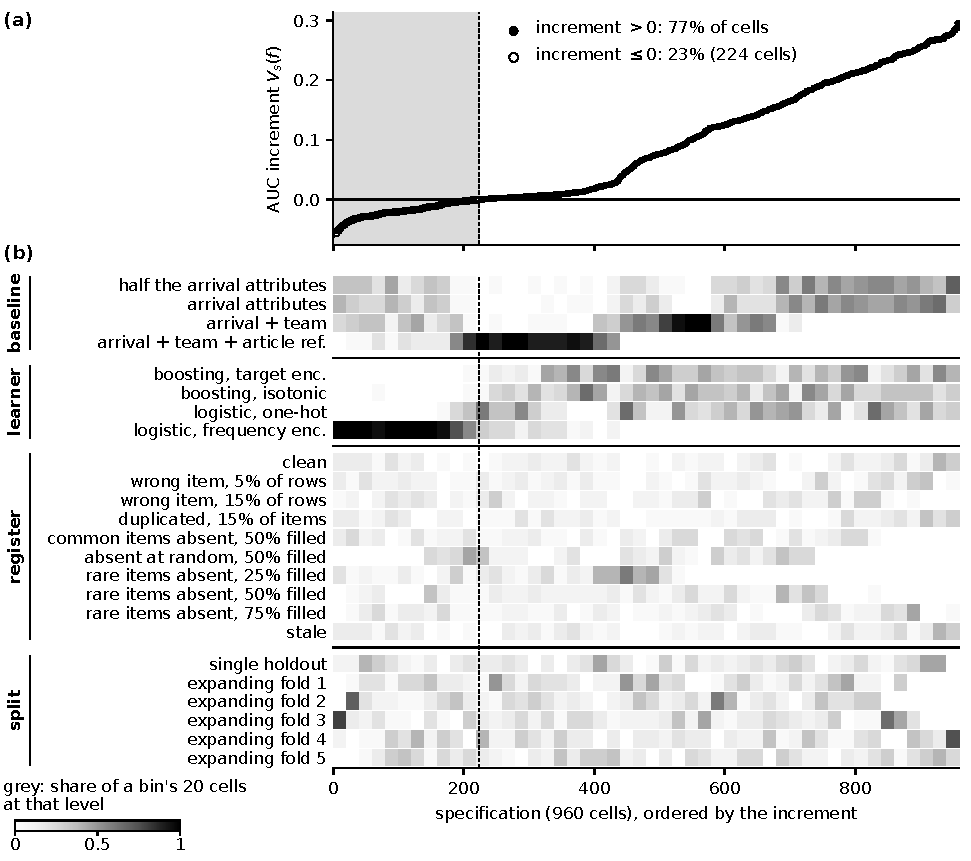
\includegraphics[width=\linewidth]{figS1_speccurve.pdf}
\caption{The specification curve for the configuration item on BPI Challenge 2014 (BPIC14), at the
pre-specified handover target, in the primary metric, the area under the ROC curve (AUC):
\nPipelineLevelsCase\ pipelines $\times$ \nRungsFigOne\ nested baselines
$\times$ \nQualityFigOne\ register-quality conditions $\times$ \nSplits\
splits. The other metrics are not on a common scale with AUC
(Remark~\ref{prop:nonid}). \textbf{(a)} Each admissible specification, sorted
by its increment: filled if positive, open on the shaded band if not.
\textbf{(b)} For each level of each axis, the share of the cells in each
sorted bin that sit at that level; the dashed line marks the sign change. The
intercept-only baseline is excluded. Point estimates only; the region counts
the simultaneous bands decide are in Table~\ref{tab:master}.}
\label{fig:speccurve}
\end{figure}

\paragraph{Contributions}
\begin{enumerate}
\item \textbf{An estimand for nested forecast comparisons that includes the
evaluation design.} The incremental score as a function of the benchmark,
the model class, the sample split, the forecast origin, the predictor's data
quality and the scoring rule, over a design space the reader can enumerate
(Table~\ref{tab:axes}); and an exact functional-ANOVA decomposition of its
variance in which the evaluation split is an \emph{error stratum}, so that
the evaluation split, with its sampling variability and fold-to-fold
instability, is separated from the forecaster's other choices
(Section~\ref{sec:sobol}).
\item \textbf{Simultaneous inference over a declared family.} Max-$t$ bands
from a bootstrap that refits the forecasting models in every draw, at a
critical value that attains \covEmpHeavyWholeAtDesign\ family-wise coverage
in a simulation matched to this design (Section~\ref{sec:simband}) --- an
upper bound, because that simulation's bootstrap is ideal --- and \emph{resolution
regions}, which state where the sign of the improvement is determined, with a
robustness index $\rho$ under a declared minimum resolved share. Along the
way, refitting a high-cardinality predictor inside each draw is shown in
simulation to break the percentile bootstrap interval, which is why every
interval here is the basic one (Section~\ref{sec:boot}).
\item \textbf{Evidence on \nPairs\ pre-specified forecasting tasks and a
service-desk case study in which the forecast origin is part of the
estimand.} One frozen pipeline is run on every log--target pair a pre-specified
protocol admits, not only those where the answer resolves, and every corpus
statistic is reported on all \nPairs\ and on the \nItsmPairs\ IT-service
pairs (Supplement~\ref{sec:family}). In the case study
(Section~\ref{sec:cmdb}) the predictor's increment is large when the
reassignment forecast is issued at first touch and indistinguishable from
zero at incident creation once the benchmark holds the fields assumed recorded
by then; a decision-based evaluation prices what reading the wrong benchmark
costs a desk (Section~\ref{sec:nbregret}).
\end{enumerate}

\noindent Figure~\ref{fig:overview} summarises the method.
\emph{Specification regret}, what choosing one specification costs against
the best, is a robustness check only; it is null on this corpus
(Supplement~\ref{sec:regretdef}).

\begin{figure}[!t]
\centering
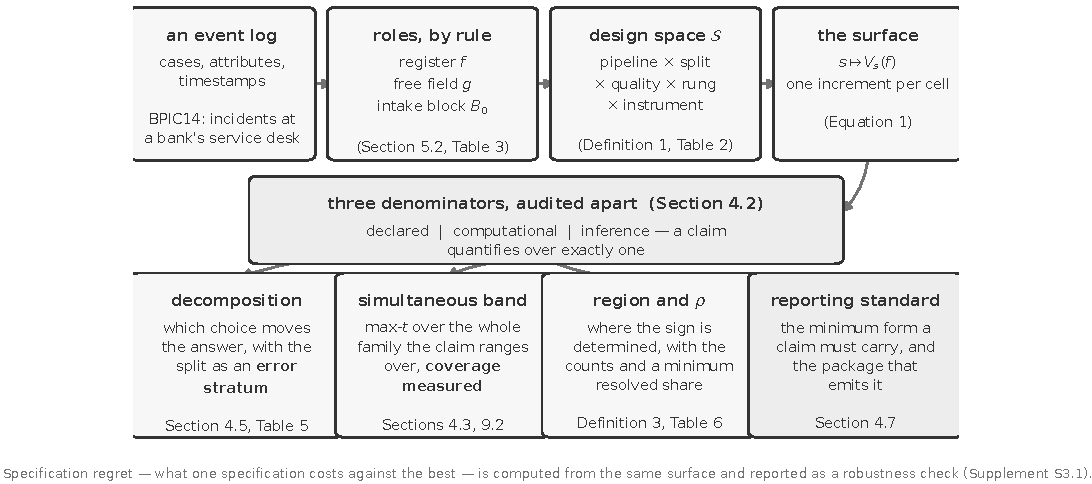
\includegraphics[width=\linewidth]{figS8_overview.pdf}
\caption{The method, once. A log is read into three \emph{roles} by declared
rules; the roles are crossed over a declared \emph{design space}; the result
is a \emph{surface}, one increment per cell. Every claim about that surface
names which of three \emph{denominators} it quantifies over, and the reporting
objects are computed from it. Each box names the section or table in which
its object is defined and reported.}
\label{fig:overview}
\end{figure}

\begin{table}[t]
\centering
\footnotesize
\setlength{\tabcolsep}{4pt}%
\renewcommand{\arraystretch}{1.2}%
\begin{tabular}{>{\raggedright\arraybackslash}p{0.17\linewidth}>{\raggedright\arraybackslash}p{0.27\linewidth}cc>{\raggedright\arraybackslash}p{0.26\linewidth}}
\toprule
object & what it is for & \S & table & what it costs \\
\midrule
Sensitivity decomposition & how much of the disagreement each analysis choice explains, and how much belongs to no single one & \ref{sec:sobol} & \ref{tab:sobol} & exact; no refit. A M\"obius sum over the surface already computed \\
Simultaneous band & an interval that holds over every cell a claim quantifies over, not one cell at a time & \ref{sec:simbands} & \ref{tab:calbands} & the whole cost: one draw refits every arm of every cell \\
Resolution region and $\rho$ & which way the surface points where the data settle it, and how much of it they settle & \ref{sec:regionsdef} & \ref{tab:triple} & a function of the band; no further refit \\
Specification regret \emph{(a check, not an object)} & what choosing one specification costs against the best one, on a scale a decision can use --- it returns a null on this corpus & \ref{app:regretfull} & \ref{tab:rules} & exact; no refit, on the surface already computed \\
\bottomrule
\end{tabular}
\caption{\textbf{The reporting objects.} The three this paper supplies and the fourth it retains as a robustness check, what each is for, where it is defined, where it is reported on this corpus, and what it costs; the two middle columns are the section it is defined in and the table that reports it. Only the second costs model fits: a draw of the bootstrap refits every arm of every cell, which is why the surface an inference is taken over is smaller than the surface a point estimate is taken over (Section~\ref{sec:threesurfaces}). The other three are functions of a surface that has already been computed, so an analyst who has done the sweep has already paid for them.}
\label{tab:objects}
\end{table}


\paragraph{Scope and supplement}
This is a retrospective study on public data, offered as a forecast
evaluation methodology; it is not a systematic review of reporting practice
or a report of a deployed forecasting system, and Section~\ref{sec:lim} says
what each would have required. The protocol and its amendments, the proofs,
the correction register and the tables this article does not print are in a
supplementary document whose sections, tables and figures carry an
\textsf{S}; Supplement~\ref{app:glossary} is a glossary of every term used
here in a technical sense.

\section{Related work}
\label{sec:related}

In the forecasting literature the incremental question is asked of one
evaluation design at a time. Whether one forecast is more accurate than
another is tested by \citet{diebold1995comparing} and
\citet{west1996asymptotic}; whether a predictor adds accuracy to a model that
nests the one without it --- the incremental question, exactly --- by
\citet{clark2001nested}, and \citet{clark2007approximately} show that under
the null, estimating the larger model's extra parameters inflates its
out-of-sample mean squared error, biasing the raw comparison against it;
whether it adds accuracy \emph{conditionally}, at a given origin and state,
by \citet{giacomini2006conditional}. \citet{gonzalo2024outofsample} extend
nested out-of-sample comparison to many candidate predictors at once, and
\citet{liu2024marginal} measure the marginal predictive content of predictor
groups across targets and horizons; both vary the predictor and hold the
evaluation design fixed, where this paper holds the predictor fixed and
varies the design. Probability forecasts of a binary event are evaluated in
the area under the ROC curve \citep{lahiri2013evaluating}, in which a
predictor's increment over a nested baseline is read
\citep{liu2016recessions} and tests of that increment are badly behaved at
the null \citep{demler2012misuse,pepe2013testing} --- one reason the
increments here are reported as estimates with intervals, although deciding
a sign still operates at that null --- and in proper scores
\citep{brier1950verification,gneiting2007scoring}, whose decomposition
separates the calibration an AUC ignores from the discrimination it measures
\citep{dimitriadis2021stable}. Reliability, ROC and Murphy curves together
separate calibration, discrimination and value when probabilistic
classifiers are compared \citep{dimitriadis2024triptych}; this paper evaluates the
increment between two nested forecasts across a design, and
Section~\ref{sec:dca} reads that increment in net benefit.

Several of the choices this paper puts on a surface have been studied one at
a time: the estimation window, over which \citet{rossi2012window} make tests
robust; the sample split, whose choice \citet{hansen2012sample} show can
manufacture rejections, and whose place in the limit theory of nested
comparisons \citet{hansen2015equivalence} characterise through Wald
statistics; the forecast origin, along which \citet{giacomini2010unstable}
track relative performance and which rolling-origin evaluation varies by
design \citep{tashman2000outofsample}; and the accuracy measure, which can
change which forecast is best \citep{hyndman2006another,kolassa2020best}.
Applied forecasters meet the joint dependence: whether the Phillips curve
helps forecast euro-area inflation turns on the specification chosen, and
averaging over modelling choices helps \citep{banbura2023phillips}.
\citet{petropoulos2022forecasting} and \citet{hewamalage2023forecast} collect
the evaluation practice these rest on. When the comparison ranges over a
\emph{family} of specifications, the reality check \citep{white2000reality},
the test for superior predictive ability \citep{hansen2005spa} and the model
confidence set \citep{hansen2011mcs} control the search: the first two ask
whether the best member of a family beats a benchmark once the search is
accounted for, the third returns the set of members not rejected as inferior
at a declared level; and \citet{hunt2022insample} shows that pseudo-out-of-sample
tests do not keep a stable family-wise error rate when models are searched
for. This paper sits beside the family tests and takes a different object
from them: not whether the family contains a member that beats the
benchmark, nor which members survive, but the shape of a fixed predictor's
increment across the family --- how much of its variation is the
forecaster's and how much is resampling, where its sign is determined, and
how far its members sit from the one that would conventionally be reported.
A forecaster's usual answer to many specifications is to combine them
\citep{wang2023combinations}; this paper asks the prior question of how much
they disagree, and where. Forecasting also has precedents for working over the
specification space rather than at a single specification: recursive selection over
every subset of candidate regressors at each forecast origin, to ask whether
predictability survives the search \citep{pesaran1995predictability}, and
thick modelling, which keeps and combines the forecasts of many
specifications instead of selecting one
\citep{granger2004thick,aiolfi2005model}. Both use the space to produce a
forecast; this paper uses it to report how an increment varies across it.

What a forecast is worth to a decision, as distinct from how accurate it is,
is the subject of \citet{murphy1993good} and \citet{granger2000economic}, and
the with-versus-without question is asked of many objects: of a dataset,
through a betting market \citep{maymin2019wage}; of a new data source in
customer-churn forecasting, in accuracy and in campaign profit
\citep{decaigny2020incorporating}; of a member of a forecast ensemble, by
leave-one-out and Shapley differences \citep{kim2026beyond}; of individual
predictors, whose contributions to out-of-sample loss a performance-based
Shapley value attributes \citep{borup2022anatomy}; and of a step in a
forecasting process, as forecast value added \citep{fildes2025forecast}. Each
answers under one evaluation design; none asks how the answer moves when the
design moves. The clinical-prediction literature has argued for two decades
that the increment in the area under the ROC curve from adding a marker
depends on the existing model and is a poor guide to usefulness
\citep{pencina2008evaluating,cook2007roc,kerr2011evaluating}, and decision
curves read net benefit across an exchange rate
\citep{vickers2006dca,vickers2016net}, which is why the operating point is an
axis here. Multiverse and specification-curve analysis
\citep{steegen2016increasing,simonsohn2020specification} supply the sweep over
analytic choices from which the robustness index below is derived.
Incompletely recorded inputs are a forecasting problem in their own right
\citep{wen2024wind}; the register-quality axis puts the predictor's
completeness inside the estimand rather than in preprocessing. And the
forecast origin turns what machine learning treats as leakage
\citep{kaufman2012leakage,kapoor2023leakage} into a declared choice of
information set. Variable importance and data valuation, underspecification
and predictive multiplicity, many-analysts studies, and the business-process
analytics literature from which the data come, where such case-level
forecasts are called outcome-oriented predictive monitoring
\citep{teinemaa2019outcome}, are discussed in Supplement~\ref{app:related}.

\paragraph{What is new for forecast evaluation}
Forecast-comparison tests either fix the evaluation design and ask whether a
predictor, or the best of a family of models, improves accuracy
\citep{clark2001nested,hansen2005spa,gonzalo2024outofsample}, or robustify
one design choice at a time \citep{rossi2012window,hansen2012sample}. This
paper reports how a fixed predictor's incremental accuracy varies jointly
across the design, separates the evaluation split's share of that variation
from the forecaster's other choices, and gives inference that holds jointly
over a declared family. Three things are
new. The estimand is declared completely: the forecast origin and the
predictor's data quality are arguments of it rather than preliminaries, and
the measure over the design is stated rather than implied by whichever cells
were enumerated, which moves the answer (Section~\ref{sec:axes2}). The
decomposition treats the evaluation split as an error stratum and so
partitions the forecaster's choices from the split's exactly; separating
specification-induced from sampling variation has precedents ---
extreme-bounds analysis, which reports an estimate's range across
specifications \citep{leamer1983con}, multimodel analysis that attributes an
estimate's variation to each modelling choice \citep{young2017model},
functional ANOVA over a configuration space \citep{hutter2014efficient}, and
the error strata of classical experimental design --- and what is added is
its exact application to a nested out-of-sample forecast comparison, with
the evaluation split as the stratum. And the share of specifications with an
improvement in a declared direction, which is standard specification-curve
practice \citep{simonsohn2020specification} and which the robustness index
$\rho$ counts, is taken under a \emph{simultaneous} band over a declared
family rather than a pointwise test, over a counted set of specifications,
and subject to a minimum resolved share below which no direction is reported;
Section~\ref{sec:sca} and Supplement~\ref{app:sca} measure where a
specification curve's verdict and a region label part company, and
Section~\ref{sec:results-regret} measures how far the conventional report
sits from the resolved specifications. The contribution is not the
observation that a single number is usually reported. It is that an
incremental-performance claim is a functional of a declared design, that the
functional can be estimated with quantified uncertainty, and that on this
corpus it varies widely.
